\documentclass[runningheads]{llncs}

\usepackage{graphicx}
\usepackage{amsmath,amssymb}
\usepackage{booktabs}
\usepackage{multirow}
\usepackage{array}
\usepackage[table]{xcolor}
\usepackage{pifont}
\usepackage{hyperref}
\usepackage{listings}
\usepackage{tikz}
\usepackage{pgfplots}
\pgfplotsset{compat=1.18}
\usetikzlibrary{shapes.geometric, arrows.meta, positioning, calc, fit, backgrounds}

% Color definitions
\definecolor{checkgreen}{HTML}{2E7D32}
\definecolor{crossred}{HTML}{C62828}
\definecolor{ourgreen}{HTML}{E8F5E9}
\definecolor{headergray}{HTML}{ECEFF1}
\definecolor{accentblue}{HTML}{1565C0}
\definecolor{boxgray}{HTML}{F8F9FA}

% Publication palette for charts
\definecolor{color_symcode}{HTML}{3867D6}       % Royal Slate Blue
\definecolor{color_symplan}{HTML}{10AC84}       % Vibrant Emerald Green
\definecolor{color_plan}{HTML}{FA8231}          % Warm Sunset Coral
\definecolor{color_contract}{HTML}{8854D0}      % Deep Wisteria Purple
\definecolor{chart_grid}{HTML}{E2E8F0}          % Soft Slate for Grid
\definecolor{chart_text}{HTML}{2D3748}          % Charcoal for Text

\newcommand{\cmark}{\textcolor{checkgreen}{\ding{51}}}
\newcommand{\xmark}{\textcolor{crossred}{\ding{55}}}

\lstdefinestyle{promptstyle}{
  basicstyle=\ttfamily\scriptsize,
  backgroundcolor=\color{boxgray},
  frame=single,
  rulecolor=\color{black!30},
  breaklines=true,
  columns=fullflexible,
  keepspaces=true,
  xleftmargin=1.5mm,
  xrightmargin=1.5mm
}

\begin{document}

\title{SymPlan: Enhancing Neurosymbolic Mathematical Reasoning in Compact Language Models via Representation and Planning}
\titlerunning{SymPlan: Neurosymbolic Reasoning in SLMs}

% -----------------------------------------------------------------------------
% Double-Blind Submission for AMI 2026 (Springer CCIS)
% Note: Author names and affiliations are omitted for peer review.
% -----------------------------------------------------------------------------
\author{Anonymous Author(s)}
\authorrunning{Anonymous et al.}
\institute{Paper under double-blind review for AMI 2026}

% -----------------------------------------------------------------------------
% Camera-Ready Version (Uncomment for final submission):
% \author{Tay Bui\inst{1,2}\orcidID{0009-0000-0000-0000} \and
% Huy N. G. Pham\inst{1,2}\orcidID{0009-0000-0000-0000} \and
% Nhan Ha Le Thanh\inst{3}\orcidID{0009-0000-0000-0000}}
% \authorrunning{T. Bui et al.}
% \institute{University of Information Technology, Ho Chi Minh City, Vietnam \and
% Vietnam National University, Ho Chi Minh City, Vietnam \and
% FPT University, Ho Chi Minh City, Vietnam\\
% \email{\{24521589, 24520690\}@gm.uit.edu.vn, hnhan5355@gmail.com}}
% -----------------------------------------------------------------------------

\maketitle

\begin{abstract}
Mathematical reasoning with language models increasingly relies on executable symbolic programs, yet monolithic program synthesis---which asks a model to simultaneously parse linguistic problem descriptions, formulate algebraic solution plans, and write formal code in a single prompt---imposes an excessive cognitive load on compact small language models (SLMs, $\le 8\text{B}$ parameters). While monolithic methods such as SymCode are effective for large, highly parameterized models, compact backbones under resource-constrained settings (e.g., 4-bit quantization) frequently suffer from semantic misformulation, domain boundary omission, and silent regressions during self-repair. We introduce SymPlan, an inspectable neurosymbolic framework specifically tailored to provide the structural scaffolding needed by compact language models. SymPlan decouples problem solving into three coordinated, contract-governed phases: (1) a \textit{Fused Target-Planning Phase} that extracts an explicit target specification, an output type contract, and an algorithmic SymPy roadmap in a single bounded inference step ($\le 256$ tokens); (2) \textit{Contract-Guided SymPy Generation} that guides deterministic code synthesis toward satisfying domain invariants; and (3) \textit{Targeted Debugging with Anti-Regression Selection}, which couples AST static diagnostics with a conservative ranking heuristic designed to reduce the risk of later repair iterations overwriting valid intermediate predictions. Evaluated across six diverse open-weight small language models (3B to 8B parameters) on the full MATH-500 benchmark under 4-bit quantization, SymPlan demonstrates that explicit representation and contract enforcement make neurosymbolic reasoning reliable and robust on compact backbones, achieving consistent gains of $+3.60\%$ to $+5.20\%$ (averaging $+4.20\%$) over monolithic SymCode and $+12.64\%$ over Chain-of-Thought, alongside a $+6.07\%$ increase in Execution Success Rate ($89.90\%$), all without parameter fine-tuning. Our findings indicate that rather than increasing parameter scale, introducing disciplined interfaces between mathematical intent and symbolic execution provides the right architectural fit to unlock dependable reasoning on compact models.

\keywords{Neurosymbolic Reasoning \and Mathematical Problem Solving \and Small Language Models \and SymPy Code Generation \and Algorithmic Planning.}
\end{abstract}

\section{Introduction}

Large Language Models (LLMs) have demonstrated strong capabilities in complex reasoning tasks, with Chain-of-Thought (CoT) prompting improving their ability to perform multi-step reasoning~\cite{wei2022cot}. Subsequent methods improve robustness by sampling multiple reasoning paths, decomposing difficult questions into simpler subproblems, or constructing an explicit plan before solving~\cite{wang2023selfconsistency,zhou2023leasttomost,wang2023plan}. However, autoregressive mathematical reasoning remains susceptible to calculation errors, missing reasoning steps, and semantic misunderstandings, making intermediate solutions difficult to reliably inspect or verify~\cite{lyu2023faithful,lightman2024verify}.

Program-aided approaches address these limitations by delegating computation to executable programs. Program-Aided Language Models (PAL)~\cite{gao2023pal} and Program-of-Thought (PoT)~\cite{chen2022pot} separate reasoning from computation by using external interpreters for numerical operations. MathCoder and ToRA further integrate natural-language reasoning with code execution and mathematical tools~\cite{wang2024mathcoder,gou2024tora}. More recently, SymCode~\cite{nezhad2025symcode} extends this paradigm to symbolic mathematics by generating executable programs with the SymPy symbolic computation library~\cite{meurer2017sympy}, enabling mathematical solutions to be checked through program execution.

\begin{figure}[t]
\centering
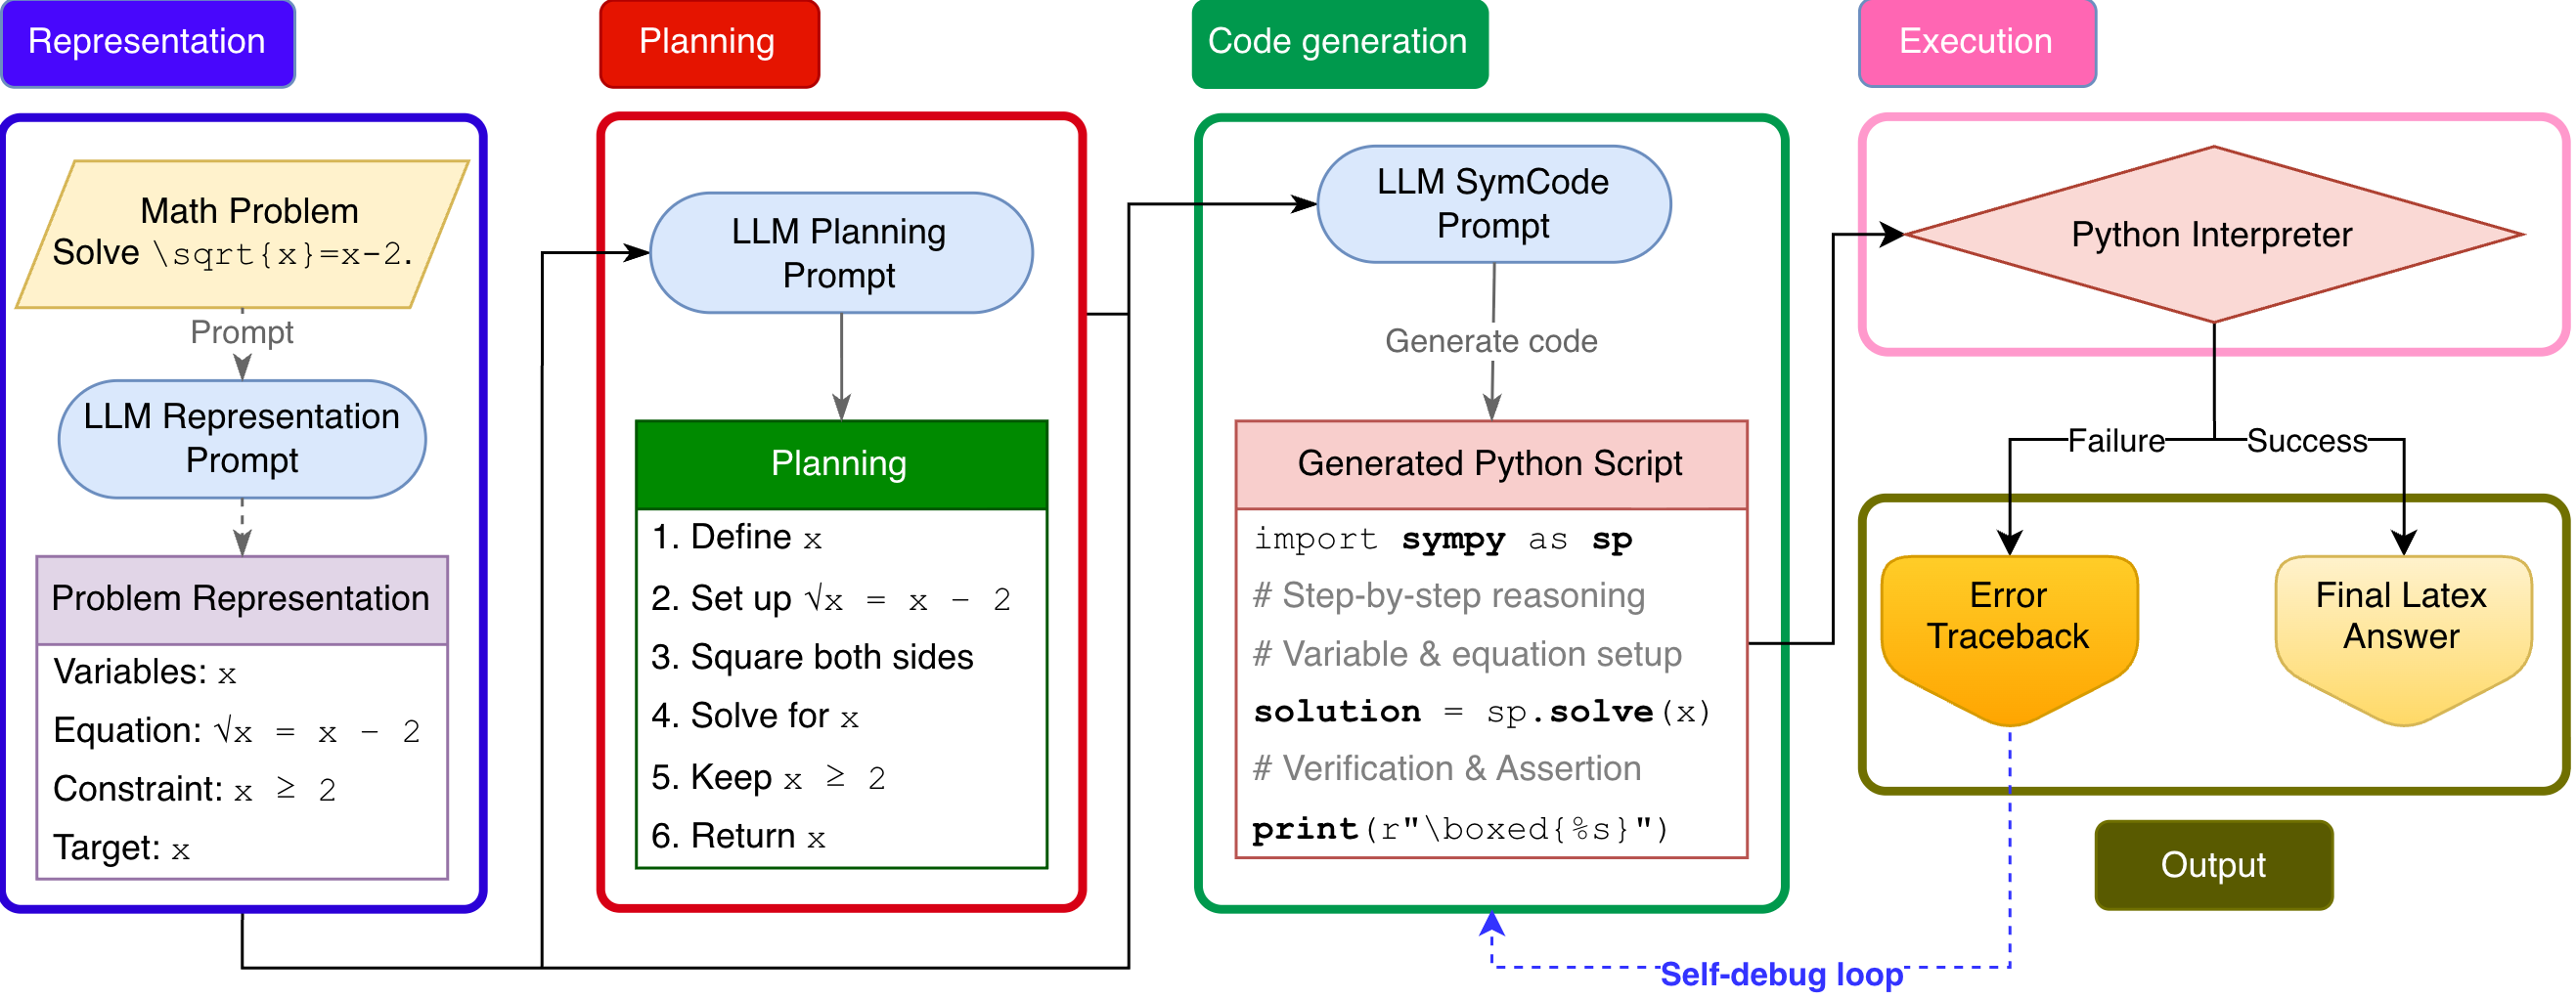
\includegraphics[width=\textwidth]{pipeline-symplan.png}
\caption{Overview of SymPlan. A problem is transformed into a fused target specification, output contract, and plan before contract-guided SymPy code generation. The script is executed by a Python interpreter; failures return traceback and static diagnostics to code repair, while successful runs produce the final \LaTeX{} answer.}
\label{fig:overview}
\end{figure}

Despite these advances, program execution alone does not guarantee correct problem interpretation. Translation-based neurosymbolic systems fundamentally depend on the correctness of the generated formalization before a deterministic solver is invoked~\cite{lyu2023faithful,pan2023logiclm}. Existing program-aided approaches typically couple problem understanding, solution reasoning, and program synthesis within a single monolithic generation process~\cite{gao2023pal,nezhad2025symcode}. While this unified strategy is viable for large-scale frontier models with substantial parameter reserves, it overburdens compact small language models ($\le 8\text{B}$ parameters), which must simultaneously parse complex mathematical prose, formulate a multi-step algebraic strategy, and satisfy strict symbolic library APIs. Although hierarchical decomposition and planning can reduce missing-step errors~\cite{khot2023decomposed,zhou2023leasttomost,wang2023plan}, they have not been systematically integrated with target typing contracts and execution-guided repair in symbolic code generation for resource-constrained models.

To investigate these challenges, we conduct a systematic failure analysis across six representative compact language models---Qwen2.5-3B-Instruct, Qwen3-4B, Qwen2.5-7B-Instruct, Qwen2.5-Coder-7B-Instruct~\cite{hui2024qwen25coder,qwen2024qwen25}, Llama-3.1-8B-Instruct~\cite{dubey2024llama3}, and Qwen3-8B~\cite{qwen2024qwen25}---under 4-bit NormalFloat4 quantization~\cite{dettmers2023qlora} on the complete MATH-500 benchmark~\cite{lightman2024verify,hendrycks2021math}, using SymPy~\cite{meurer2017sympy} as the symbolic computation engine. Across these diverse models, we observe that monolithic generation creates cognitive overload for smaller backbones, manifesting in four recurring failure patterns: (1) \textit{semantic misformulation}, where executable code solves an unprompted or distorted problem; (2) \textit{target contract violation}, such as enumerating candidate elements when asked for an integer count, or producing floating-point approximations instead of exact fractions; (3) \textit{domain constraint omission}, leading to the acceptance of extraneous or out-of-domain roots; and (4) \textit{silent repair regression}, where standard iterative debugging produces a runnable script that accidentally overwrites a previously correct answer with a degraded prediction.

Motivated by these findings, we propose SymPlan, an inspectable, planning-guided neurosymbolic framework designed specifically to provide the structural scaffolding required by compact language models. Rather than burdening the model with one-shot code generation, SymPlan introduces three coordinated stages that match the processing capacity of SLMs. First, a \textit{Fused Target-Planning Phase} extracts a formal target specification, an explicit output contract, and a step-by-step computational plan in a single bounded call, eliminating multi-turn context drift. Second, a \textit{Contract-Guided Code Generator} translates this specification into a self-contained, deterministic SymPy script that enforces exact arithmetic and domain boundary filters. Third, a \textit{Targeted Debugging Loop} couples interpreter feedback and static AST diagnostics with an \textit{Anti-Regression Selection} mechanism, which evaluates all historical execution attempts to provide a conservative mechanism for retaining the strongest verified execution candidate across repair iterations.

Our contributions are as follows:
\begin{enumerate}
    \item We present a comprehensive empirical characterization of formulation, contract, and debugging failure modes in monolithic symbolic reasoning across six compact language models on the full MATH-500 benchmark, identifying the specific bottlenecks where unguided generation overburdens small backbones.
    \item We introduce SymPlan, an open-source neurosymbolic framework tailored to compact models that combines fused representation-planning, contract-guided SymPy code generation, and anti-regression attempt ranking.
    \item We demonstrate that structured decomposition is particularly well-suited to compact models: across six open-weight backbones (3B--8B), SymPlan yields stable, universal accuracy improvements ($+3.60\%$ to $+5.20\%$ over monolithic SymCode and $+12.64\%$ over Chain-of-Thought) and improves execution success by $+6.07\%$, showing that small models can achieve dependable symbolic reasoning when provided with explicit contract scaffolding.
\end{enumerate}

\section{Related Work}

\subsection{Mathematical Reasoning}

Chain-of-Thought (CoT) prompting elicits intermediate natural-language rationales and substantially improves arithmetic, commonsense, and symbolic reasoning in sufficiently capable language models~\cite{wei2022cot}. Zero-shot and few-shot extensions seek to make this reasoning more reliable without modifying model parameters. Self-consistency samples multiple reasoning trajectories and selects their majority answer~\cite{wang2023selfconsistency}, while Least-to-Most prompting first decomposes a difficult question into simpler dependent subproblems~\cite{zhou2023leasttomost}. Plan-and-Solve similarly asks the model to construct and then execute a solution plan, reducing missing-step and calculation errors~\cite{wang2023plan}.

These methods improve answer accuracy, but their intermediate text is neither executable nor necessarily faithful to the computation that produced the final prediction~\cite{lyu2023faithful}. This distinction is particularly critical in mathematics: a fluent derivation can harbor an early semantic misinterpretation, an omitted domain condition, or an invalid algebraic transformation whose consequences propagate through every subsequent step. Process supervision and step-level verification can identify some local errors~\cite{lightman2024verify}, while specialized mathematical foundation models such as DeepSeekMath~\cite{shao2024deepseekmath} and Qwen2.5-Math~\cite{yang2024qwen25math} demonstrate substantial gains through domain pretraining. Concurrently, highly capable small language models such as Phi-3~\cite{abdin2024phi3} show that compact models can achieve competitive reasoning efficiency when provided with structured prompting. SymPlan bridges these directions by focusing specifically on the interface between informal problem interpretation and symbolic execution, providing the structural scaffolding necessary for compact models to conduct reliable neurosymbolic reasoning without parameter updates.

\subsection{Program-Aided Reasoning}

Program-aided methods treat executable code as an intermediate representation, allowing an external interpreter to perform exact or repeated computation. PAL delegates computational steps to generated programs while retaining the model for semantic reasoning~\cite{gao2023pal}; PoT similarly separates the formulation of a solution from numerical execution~\cite{chen2022pot}. MathCoder interleaves natural language, code, and execution results through code-integrated mathematical training~\cite{wang2024mathcoder}, whereas ToRA learns interactive trajectories that combine textual reasoning with calculators, computation libraries, and symbolic solvers~\cite{gou2024tora}. These approaches demonstrate that tool use can reduce arithmetic burden and extend the range of solvable problems.

For symbolic mathematics, SymCode directly generates programs using SymPy~\cite{nezhad2025symcode,meurer2017sympy}. This supports exact algebra, calculus, equation solving, and modular arithmetic beyond ordinary numerical Python. However, executable code provides a certificate only for what the program actually computes. If the model encodes the wrong equation, returns an intermediate quantity, or omits a domain restriction, the interpreter may report success while the mathematical answer remains incorrect. Such risks grow for compact models because code generation adds syntax, library selection, typing, and output-formatting requirements to the original reasoning task.

\subsection{Neurosymbolic Formalization}

Neurosymbolic frameworks use language models to translate informal inputs into formal structures that deterministic systems can execute. Faithful CoT separates translation into a symbolic reasoning chain from deterministic problem solving~\cite{lyu2023faithful}. Logic-LM translates natural-language logic problems into solver-compatible formulations and uses solver feedback to refine invalid translations~\cite{pan2023logiclm}. These systems improve faithfulness by making the solver's contribution explicit, but they also reveal a central bottleneck: deterministic inference cannot recover information that was omitted or mistranslated during formalization.

SymPlan shares this translation--execution perspective but specifically addresses the resource and parameter constraints of compact open-weight models. Rather than moving directly from an informal question to a complete formal program, it introduces a fused contract defining target specifications, output type constraints, and an implementation-independent symbolic plan. This design reduces cognitive load on the language model before it encounters the strict syntactic and API requirements of executable SymPy code.

\subsection{Planning and Verification}

Task decomposition provides a complementary route to reliable reasoning. Decomposed Prompting delegates complex problems to modular subtask prompts~\cite{khot2023decomposed}; Least-to-Most solves a sequence of increasingly dependent subproblems~\cite{zhou2023leasttomost}; and Plan-and-Solve separates plan construction from plan execution~\cite{wang2023plan}. Their plans are generally expressed in free-form language, however, and therefore do not by themselves guarantee that variables, constraints, and output targets survive the transition to executable code.

Execution feedback can repair a different class of failures. Self-Debugging and iterative refinement show that language models can inspect generated programs, execution results, and error messages to revise faulty code~\cite{chen2024selfdebug,madaan2023selfrefine}. Logic-LM similarly uses symbolic-solver errors for self-refinement~\cite{pan2023logiclm}. Such feedback is highly informative for syntax, API, and type errors, but a runnable program may provide no traceback even when its mathematical formulation is wrong. SymPlan therefore combines execution-guided repair with a fixed representation and plan: tracebacks may revise implementation details, while the explicit mathematical state anchors the intended semantics across debugging attempts.

\section{Method}
\label{sec:method}

\subsection{Framework Overview}

Given a natural-language mathematical problem $q$, monolithic program-aided approaches such as SymCode~\cite{nezhad2025symcode} synthesize and execute an end-to-end Python script in a single step:
\begin{equation}
C_{\text{base}} \sim \mathcal{M}(\cdot \mid q), \quad \hat{y} = \operatorname{Exec}(C_{\text{base}}).
\end{equation}
While straightforward, this formulation requires the model to simultaneously parse linguistic context, identify mathematical targets, select a computational algorithm, and satisfy formal library APIs. For compact language models ($\le 8\text{B}$ parameters), this unconstrained generation frequently results in semantic misformulation, domain omission, and silent regressions during repair.

To resolve these compounding failure modes, SymPlan decouples symbolic problem solving into three coordinated, contract-governed phases:
\begin{align}
\mathcal{T} = (\tau, \Omega, \mathcal{P}) &= \operatorname{FusedPlan}_{\mathcal{M}}(q), \label{eq:fused_plan} \\
C^{(0)} &= \operatorname{CodeGen}_{\mathcal{M}}(q, \tau, \Omega, \mathcal{P}), \label{eq:codegen} \\
\mathcal{H} &= \operatorname{ExecuteAndRepair}_{\mathcal{M}}(C^{(0)}, q, \tau, \Omega, \mathcal{P}), \label{eq:repair} \\
\hat{y} &= \operatorname{SelectBest}(\mathcal{H}, \Omega), \label{eq:select}
\end{align}
where $\tau$ is the explicit target specification, $\Omega$ denotes the output type contract, $\mathcal{P}$ is the ordered symbolic plan, and $\mathcal{H}$ is the history of execution attempts. By freezing the problem contract before code synthesis and maintaining a structured evaluation of attempt history, SymPlan reduces semantic drift across repair iterations without requiring iterative human guidance.

\subsection{Fused Target Extraction and Algorithmic Planning}
\label{sec:fused_planning}

\textbf{Motivation.} Prior neurosymbolic systems often rely on multi-turn dialogue pipelines that separate entity extraction from strategic planning~\cite{lyu2023faithful,khot2023decomposed}. However, our preliminary investigations on compact SLMs revealed that chaining distinct prompting turns exacerbates cumulative context drift, doubles autoregressive generation latency, and increases instruction dropouts. Conversely, unguided code generation lacks explicit output invariants, causing models to return raw coordinate sets when asked for an integer count, or decimal approximations when exact symbolic expressions are required.

\textbf{Module Design.} SymPlan introduces a \textit{Fused Target-Planning Phase} executed in a single, strictly bounded inference step ($\le 256$ tokens). Given problem $q$, the model emits a structured contract tuple $\mathcal{T} = (\tau, \Omega, \mathcal{P})$ without computing intermediate arithmetic:
\begin{itemize}
    \item \textbf{Target Specification ($\tau$):} The formal mathematical quantity or relation queried by the prompt (e.g., ``the number of positive real roots'', ``the coordinates of the center'').
    \item \textbf{Output Type Contract ($\Omega$):} A categorical type contract $\Omega \in \{\texttt{number}, \texttt{text}, \texttt{tuple}, \texttt{set}, \texttt{symbolic}\}$. For instance, if the prompt asks ``how many'', $\Omega$ specifies a \texttt{number} representing cardinality ($\operatorname{card}(S)$), instructing the model to return the scalar count rather than enumerating the raw solution set $S$.
    \item \textbf{Computational Plan ($\mathcal{P}$):} An ordered sequence of symbolic operations $\mathcal{P} = (p_1, \ldots, p_m)$, specifying symbol definitions (\texttt{sp.symbols}), equation formulations (\texttt{sp.Eq}), algebraic transformations, and domain boundary filtering.
\end{itemize}

\textbf{Technical Advantages.} Compressing target extraction and planning into a single bounded forward pass avoids the cumulative context duplication and multiple API round-trip latencies of multi-turn dialogue while establishing clear mathematical grounding before code generation. Furthermore, explicitly declaring $\Omega$ establishes a structural specification that guides subsequent code synthesis and downstream parsing.

\subsection{Contract-Guided SymPy Code Generation}
\label{sec:codegen}

\textbf{Motivation.} Monolithic code generators frequently succumb to three library-specific vulnerabilities: (1) \textit{syntax leakage}, wherein models interleave natural-language reasoning comments that pollute Python interpreter blocks; (2) \textit{domain boundary violations}, such as retaining extraneous negative roots for geometric lengths; and (3) \textit{library API misuse}, such as passing non-integer floats to \texttt{sp.Rational(p, q)} or calling \texttt{.evalf()} on fractions where exact expressions are mandated.

\textbf{Module Design.} The code generator $\operatorname{CodeGen}_{\mathcal{M}}$ consumes problem $q$ conditioned on the frozen contract $(\tau, \Omega, \mathcal{P})$ and generates a self-contained Python script using SymPy~\cite{meurer2017sympy}. The generation prompt provides systematic guidelines and few-shot demonstrations designed to encourage compliance with safe symbolic coding practices:
\begin{enumerate}
    \item \textit{Exact Symbolic Arithmetic:} All rational values are constructed via \texttt{sp.Rational(p, q)} for integers $p, q \in \mathbb{Z}$, or symbolic division \texttt{sp.S(p) / q} for radical expressions. Floating-point conversions via \texttt{.evalf()} are discouraged unless explicit decimal precision is queried, prioritizing exact symbolic expressions.
    \item \textit{Domain Filtering and Validation:} The prompt instructs the model to filter candidate roots returned by \texttt{sp.solve} against domain constraints (e.g., $x \in \mathbb{R}^+$, integer modular domains, non-zero denominators).
    \item \textit{Algebraic Simplification:} Rational expressions are canonicalized via \texttt{sp.together()} or \texttt{sp.cancel()} prior to output formatting.
    \item \textit{Standardized Canonical Output:} The script terminates with a single print statement formatting the answer into \LaTeX{} boxed notation:
\end{enumerate}
\begin{lstlisting}[style=promptstyle,language=Python]
import sympy as sp

# 1. Define symbols and domain constraints
x = sp.symbols('x', real=True)
eq = sp.Eq(sp.sqrt(x), x - 2)

# 2. Solve and filter against domain constraints (x >= 2)
candidates = sp.solve((x - 2)**2 - x, x)
valid = [s for s in candidates if s >= 2 
         and sp.simplify(eq.lhs.subs(x, s) - eq.rhs.subs(x, s)) == 0]

# 3. Emit formatted answer conforming to \Omega
print(r"\boxed{%s}" % sp.latex(valid[0]))
\end{lstlisting}

\textbf{Technical Advantages.} Because code generation is conditioned on the pre-established plan $\mathcal{P}$ and type $\Omega$, the search space is constrained to implementing verified mathematical transformations rather than simultaneously inventing the algebraic strategy.

\subsection{Targeted Debugging with Anti-Regression Selection}
\label{sec:debugging}

\textbf{Motivation.} Standard self-debugging workflows in program-aided reasoning suffer from two fundamental weaknesses on compact models: (1) \textit{code cycling}, where models repeatedly emit identical failing syntax across retries; and (2) \textit{silent semantic regression}, where a revised script executes successfully without traceback errors but silently replaces a mathematically valid intermediate result with an ungrounded hallucination.

\textbf{Module Design.} SymPlan implements a robust execution-verification loop bounded by $K=2$ repair attempts. The generated script $C^{(i)}$ is executed in an isolated Python sandbox with a strict timeout $\tau = 15$ seconds. The debugging mechanism introduces three key safeguards:
\begin{itemize}
    \item \textbf{AST Static Linting and Verification:} If execution fails or emits no parseable result, the system extracts the traceback $e^{(i)}$ and enriches it with an AST static linter (\texttt{lint\_sympy\_code}) and lightweight candidate verification diagnostics $v^{(i)}$.
    \item \textbf{Targeted Repair with Anti-Cycling:} The repair prompt receives $q$, the original plan $\mathcal{P}$, failing code $C^{(i)}$, traceback $e^{(i)}$, and verification diagnosis $v^{(i)}$. Crucially, if $C^{(i)} \equiv C^{(i-1)}$, the prompt injects an explicit constraint demanding a materially distinct implementation strategy.
    \item \textbf{Anti-Regression Record Ranking:} Rather than naively accepting the output of the final retry attempt $C^{(K)}$, SymPlan records every attempt into an episodic history $\mathcal{H} = \{r_0, \ldots, r_k\}$. Each record $r$ is evaluated via a lexicographic ranking tuple:
    \begin{equation}
    \operatorname{Rank}(r) = \langle \mathbb{I}_{\text{exec}}(r), \mathbb{I}_{\text{valid}}(r), \mathbb{I}_{\text{verif}}(r), -\operatorname{attempt}(r) \rangle,
    \end{equation}
    where $\mathbb{I}_{\text{exec}}$ indicates zero execution errors, $\mathbb{I}_{\text{valid}}$ indicates non-null boxed extraction, $\mathbb{I}_{\text{verif}}$ indicates candidate verification pass, and $-\operatorname{attempt}(r)$ favors earlier valid attempts over speculative later mutations. The optimal record is selected as:
    \begin{equation}
    r^* = \arg\max_{r \in \mathcal{H}} \operatorname{Rank}(r).
    \end{equation}
    \item \textbf{Multi-Tier Fallback Strategy:} If $r^*$ yields an unparseable or empty prediction, SymPlan executes a deterministic fallback cascade: (i) reverse-scanning raw model responses for embedded boxed expressions, (ii) extracting regex candidates from plan notes, and (iii) applying post-hoc type normalization via $\operatorname{FormatContract}(\hat{y}, \Omega)$.
\end{itemize}

\textbf{Technical Advantages.} The anti-regression ranking provides a conservative selection mechanism that substantially reduces the risk of regression across repair iterations by ensuring that a speculative later retry cannot overwrite an earlier candidate with equal or superior execution and verification status.

\section{Experiments}
\label{sec:experiments}

\subsection{Experimental Setup}

\subsubsection{Benchmark}

We evaluate all methods on MATH-500~\cite{lightman2024verify,hendrycks2021math} as a standardized diagnostic benchmark. Sampled from the competition-level MATH dataset, MATH-500 spans seven core mathematical subjects (\textit{Algebra, Intermediate Algebra, Number Theory, Counting \& Probability, Geometry, Precalculus, Prealgebra}) and five graduated difficulty levels (Level 1 through Level 5), providing a calibrated testbed to diagnose formalization and computational errors.

\subsubsection{Model and Execution Configuration}

To test scalability and architectural suitability across compact model families and parameter scales, we evaluate six representative open-weight language models spanning three parameter tiers (3B, 4B, 7B, and 8B):
\begin{itemize}
    \item \textbf{Qwen2.5-3B-Instruct} (3.09B parameters)~\cite{qwen2024qwen25}
    \item \textbf{Qwen3-4B} (4.02B parameters)~\cite{qwen2024qwen25}
    \item \textbf{Qwen2.5-7B-Instruct} (7.61B parameters)~\cite{qwen2024qwen25}
    \item \textbf{Qwen2.5-Coder-7B-Instruct} (7.61B parameters, code-specialized)~\cite{hui2024qwen25coder}
    \item \textbf{Llama-3.1-8B-Instruct} (8.03B parameters)~\cite{dubey2024llama3}
    \item \textbf{Qwen3-8B} (8.19B parameters)~\cite{qwen2024qwen25}
\end{itemize}
This selection deliberately encompasses multiple distinct architectural lineages (Qwen and Llama), including both general-purpose reasoning architectures and code-specialized backbones (Qwen2.5-Coder), establishing a diverse testbed to assess architectural suitability across different pretraining distributions. All models are evaluated under 4-bit NormalFloat4 (NF4) quantization using \texttt{bitsandbytes}~\cite{dettmers2023qlora} with Scaled Dot-Product Attention (SDPA). Across all methods, decoding is fully deterministic via greedy search: \texttt{temperature} $= 0.0$, \texttt{top\_p} $= 1.0$, and a generation ceiling of \texttt{max\_new\_tokens} $= 1024$. In-sandbox program execution is strictly enforced with a timeout threshold $\tau = 15$ seconds and a maximum retry budget $K = 2$.

\subsubsection{Baseline Methods}

We benchmark SymPlan against three established reasoning paradigms evaluated under strictly identical model quantization and runtime environments:
\begin{enumerate}
    \item \textbf{Direct:} Zero-shot direct mathematical answer generation without intermediate scratchpad steps.
    \item \textbf{Chain-of-Thought (CoT):} Step-by-step natural-language reasoning with final boxed answer extraction~\cite{wei2022cot}.
    \item \textbf{SymCode:} State-of-the-art monolithic CoT and SymPy code generation with interpreter traceback self-repair~\cite{nezhad2025symcode}.
\end{enumerate}

\subsubsection{Evaluation Metrics}

\begin{itemize}
    \item \textbf{Accuracy (\% Exact Match):} Evaluated through robust three-tier equivalence checking: (1) string canonicalization, (2) SymPy algebraic simplification $\operatorname{simplify}(\hat{y} - y) = 0$, and (3) numeric tolerance $|\hat{y} - y| < 10^{-5}$.
    \item \textbf{Execution Success Rate (ESR \%):} The fraction of generated scripts that execute to completion within $\tau=15$s without runtime exceptions and produce a parseable boxed candidate.
    \item \textbf{Average Token Cost:} The total number of generated autoregressive tokens per problem, measuring computational inference efficiency.
\end{itemize}

\subsection{Main Results}
\label{sec:results}

Table~\ref{tab:mainresults} presents the primary cross-model accuracy comparison on MATH-500, while Fig.~\ref{fig:chart} details the Execution Success Rate (ESR) across all six models.

\begin{table}[t]
\centering
\caption{Cross-model answer accuracy (\%) on the full MATH-500 benchmark across six compact models (3B--8B). Best accuracy per model is in \textbf{bold}.}
\label{tab:mainresults}
\resizebox{\columnwidth}{!}{%
\begin{tabular}{llcccc}
\toprule
\rowcolor{headergray}
\textbf{Model} & \textbf{Size} & \textbf{Direct} & \textbf{CoT} & \textbf{SymCode} & \textbf{SymPlan (Ours)} \\
\midrule
Qwen2.5-3B-Instruct & 3B & 17.00 & 39.80 & 37.40 & \textbf{41.20} \\
Qwen3-4B & 4B & 36.00 & 45.40 & 56.40 & \textbf{61.60} \\
Qwen2.5-7B-Instruct & 7B & 25.40 & 45.60 & 54.00 & \textbf{57.60} \\
Qwen2.5-Coder-7B-Instruct & 7B & 22.00 & 38.20 & 57.00 & \textbf{61.40} \\
Llama-3.1-8B-Instruct & 8B & 23.20 & 37.60 & 37.60 & \textbf{41.80} \\
Qwen3-8B & 8B & 36.20 & 45.00 & 59.80 & \textbf{63.80} \\
\midrule
\rowcolor{ourgreen}
\textbf{Average (6 Models)} & --- & 26.63 & 41.93 & 50.37 & \textbf{54.57} \\
\bottomrule
\end{tabular}}
\end{table}

\begin{figure}[b]
\centering
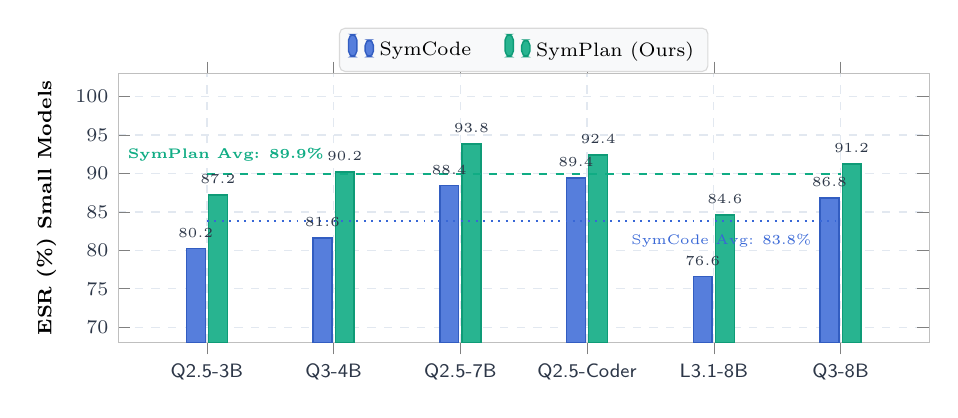
\begin{tikzpicture}
\begin{axis}[
    ybar=1.2pt,
    bar width=6.8pt,
    width=0.98\columnwidth,
    height=5.0cm,
    ymin=68,
    ymax=103,
    ytick={70, 75, 80, 85, 90, 95, 100},
    ylabel={\scriptsize\textbf{ESR (\%) Small Models}},
    symbolic x coords={Q2.5-3B, Q3-4B, Q2.5-7B, Q2.5-Coder, L3.1-8B, Q3-8B},
    xtick=data,
    enlarge x limits=0.14,
    nodes near coords,
    nodes near coords style={font=\fontsize{4.8pt}{5.5pt}\selectfont\bfseries, text=chart_text, yshift=0.5pt},
    legend style={
        at={(0.5,1.17)},
        anchor=north,
        legend columns=2,
        font=\scriptsize,
        draw=gray!30,
        fill=boxgray,
        rounded corners=2pt,
        /tikz/every even column/.append style={column sep=10pt}
    },
    grid=major,
    grid style={draw=chart_grid, line width=0.5pt, dashed},
    axis line style={draw=gray!50},
    x tick label style={font=\scriptsize\sffamily, text=chart_text},
    y tick label style={font=\scriptsize\sffamily, text=chart_text}
]
\addplot[fill=color_symcode!85, draw=color_symcode!90!black, line width=0.5pt] coordinates {
    (Q2.5-3B, 80.20) (Q3-4B, 81.60) (Q2.5-7B, 88.40) (Q2.5-Coder, 89.40) (L3.1-8B, 76.60) (Q3-8B, 86.80)
};
\addplot[fill=color_symplan!90, draw=color_symplan!90!black, line width=0.5pt] coordinates {
    (Q2.5-3B, 87.20) (Q3-4B, 90.20) (Q2.5-7B, 93.80) (Q2.5-Coder, 92.40) (L3.1-8B, 84.60) (Q3-8B, 91.20)
};
\draw[dashed, color_symplan, line width=0.7pt] (axis cs:Q2.5-3B,89.90) -- (axis cs:Q3-8B,89.90) node[pos=0.03, above=1pt, font=\fontsize{5pt}{6pt}\selectfont\bfseries, text=color_symplan] {SymPlan Avg: 89.9\%};
\draw[dotted, color_symcode, line width=0.7pt] (axis cs:Q2.5-3B,83.83) -- (axis cs:Q3-8B,83.83) node[pos=0.97, below=1pt, anchor=north east, font=\fontsize{5pt}{6pt}\selectfont, text=color_symcode] {SymCode Avg: 83.8\%};
\legend{SymCode, SymPlan (Ours)}
\end{axis}
\end{tikzpicture}
\caption{Execution Success Rate (ESR \%) comparison between SymCode and SymPlan across all six compact models on MATH-500. Dashed lines indicate the cross-model averages ($89.90\%$ vs. $83.83\%$).}
\label{fig:chart}
\end{figure}

These empirical results affirm our central thesis: monolithic symbolic generation poses a disproportionate challenge for compact models ($\le 8\text{B}$) because small models struggle to balance semantic planning and syntactic code generation simultaneously. When given structured scaffolding through explicit target contracts and algorithmic planning, small models avoid the formulation traps of monolithic generation. Relative to monolithic SymCode, SymPlan delivers consistent gains between $+3.60\%$ and $+5.20\%$ (averaging $+4.20\%$ across all six models), with the strongest gains observed on Qwen3-4B ($+5.20\%$) and Qwen2.5-Coder-7B ($+4.40\%$). Furthermore, compared to natural-language Chain-of-Thought (CoT), SymPlan achieves an average gain of $+12.64\%$ ($+23.20\%$ on Qwen2.5-Coder-7B and $+18.80\%$ on Qwen3-8B), confirming that symbolic computation provides indispensable calculation fidelity when properly guided by a structured plan.

Furthermore, as illustrated in Fig.~\ref{fig:chart}, SymPlan markedly improves the Execution Success Rate across all models, increasing the cross-model average from $83.83\%$ to $89.90\%$ ($+6.07\%$). Notably, on Llama-3.1-8B and Qwen3-4B, SymPlan elevates ESR by $+8.00\%$ and $+8.60\%$, respectively. This demonstrates that pre-specifying output contracts and encouraging compliance with exact SymPy coding rules substantially reduces syntax errors and undefined variable exceptions before code reaches the interpreter, lowering execution failures by $37.5\%$ across all models.

Regarding computational cost, SymPlan incurs a moderate $22.6\%$ increase in generated tokens over monolithic SymCode ($392.9$ vs. $320.6$ tokens per problem across all models, accounting for the fused plan of $\approx 85$ tokens and code synthesis of $\approx 308$ tokens), while delivering a $+4.20$ percentage point accuracy gain and remaining noticeably more compact than natural-language CoT ($423.7$ tokens). This trade-off is favorable: the modest token budget increase is dedicated to front-loaded structural planning and explicit contracts, which prevents costly execution failures and repeated repair iterations downstream.

\subsection{Stratified Analysis by Difficulty and Subject}

To understand where SymPlan's structured planning provides the greatest advantage, we examine fine-grained breakdowns across problem difficulty levels and mathematical subjects.

\begin{table}[t]
\centering
\caption{Accuracy (\%) by difficulty level on MATH-500 for Qwen2.5-Coder-7B and Qwen3-8B.}
\label{tab:levels}
\resizebox{\columnwidth}{!}{%
\begin{tabular}{llcccc}
\toprule
\rowcolor{headergray}
\textbf{Model} & \textbf{Level (Count)} & \textbf{Direct} & \textbf{CoT} & \textbf{SymCode} & \textbf{SymPlan (Ours)} \\
\midrule
\multirow{5}{*}{Qwen2.5-Coder-7B} 
& Level 1 (43) & 41.86 & 88.37 & 88.37 & \textbf{88.37} \\
& Level 2 (90) & 36.67 & 64.44 & 74.44 & \textbf{83.33} \\
& Level 3 (105) & 26.67 & 46.67 & 61.90 & \textbf{73.33} \\
& Level 4 (128) & 12.50 & 27.34 & 49.22 & \textbf{50.00} \\
& Level 5 (134) & 11.19 & 8.21 & 38.81 & \textbf{39.55} \\
\midrule
\multirow{5}{*}{Qwen3-8B} 
& Level 1 (43) & 81.40 & 83.72 & 86.05 & \textbf{90.70} \\
& Level 2 (90) & 72.22 & 76.67 & 70.00 & \textbf{76.67} \\
& Level 3 (105) & 42.86 & 53.33 & 63.81 & \textbf{66.67} \\
& Level 4 (128) & 20.31 & 35.16 & 58.59 & \textbf{60.94} \\
& Level 5 (134) & 7.46 & 14.18 & 42.54 & \textbf{47.01} \\
\bottomrule
\end{tabular}}
\end{table}

\begin{table}[t]
\centering
\caption{Subject-wise accuracy (\%) across seven mathematical subjects on MATH-500 for Qwen2.5-Coder-7B and Qwen3-8B. The SymPlan column is highlighted.}
\label{tab:subjects}
\resizebox{\columnwidth}{!}{%
\begin{tabular}{lcccccc}
\toprule
\rowcolor{headergray}
& & \multicolumn{2}{c}{\textbf{Qwen2.5-Coder-7B}} & & \multicolumn{2}{c}{\textbf{Qwen3-8B}} \\
\cmidrule{3-4} \cmidrule{6-7}
\rowcolor{headergray}
\textbf{Subject} & \textbf{Count} & \textbf{SymCode} & \textbf{SymPlan} & & \textbf{SymCode} & \textbf{SymPlan} \\
\midrule
Algebra & 124 & 66.94 & \textbf{76.61} & & 71.77 & \textbf{75.81} \\
Counting \& Probability & 38 & 52.63 & \textbf{57.89} & & 44.74 & \textbf{57.89} \\
Geometry & 41 & 31.71 & \textbf{34.15} & & 46.34 & \textbf{51.22} \\
Intermediate Algebra & 97 & \textbf{51.55} & 48.45 & & 50.52 & \textbf{51.55} \\
Number Theory & 62 & 66.13 & \textbf{70.97} & & 62.90 & \textbf{72.58} \\
Prealgebra & 82 & 69.51 & \textbf{75.61} & & 73.17 & \textbf{73.17} \\
Precalculus & 56 & 37.50 & \textbf{41.07} & & 46.43 & \textbf{48.21} \\
\bottomrule
\end{tabular}}
\end{table}

Table~\ref{tab:levels} highlights the performance across difficulty tiers. On moderately complex competition problems (Levels 2 and 3), SymPlan provides dramatic double-digit improvements over SymCode. For example, on Qwen2.5-Coder-7B, SymPlan surges from $74.44\%$ to $83.33\%$ on Level 2 ($+8.89\%$) and from $61.90\%$ to $73.33\%$ on Level 3 ($+11.43\%$). On the most challenging Level 5 problems, while pure symbolic solvers face intrinsic algebraic hardness, SymPlan sustains superior accuracy ($39.55\%$ vs $38.81\%$ on Qwen2.5-Coder, and $47.01\%$ vs $42.54\%$ on Qwen3-8B), substantially eclipsing pure prose CoT ($8.21\%$ and $14.18\%$).

The discipline breakdown in Table~\ref{tab:subjects} reveals that SymPlan's primary gains concentrate in \textit{Algebra} ($+9.67\%$ on Qwen2.5-Coder, $+4.04\%$ on Qwen3-8B), \textit{Counting \& Probability} ($+5.26\%$ and $+13.15\%$), and \textit{Number Theory} ($+4.84\%$ and $+9.68\%$). In these subjects, combinatorial conditions (such as modular congruences and non-negative integer selections) are easily dropped during monolithic generation; SymPlan's explicit target contract $(\tau, \Omega)$ guides the model to preserve these constraints during code generation. Note that the weighted sums across difficulty levels in Table~\ref{tab:levels} and subjects in Table~\ref{tab:subjects} ($\sum_i N_i \cdot \text{Acc}_i / 500$) strictly reconstruct the overall benchmark accuracies in Table~\ref{tab:mainresults} ($57.00\%$ and $61.40\%$ for Qwen2.5-Coder; $59.80\%$ and $63.80\%$ for Qwen3-8B).

\subsection{Component Ablation and Error Diagnostics}
\label{sec:ablation}

To measure the individual and compounding contributions of our architectural design, we isolate three variants across all six models on MATH-500: (1) \textit{Contract-Only}, which extracts the target contract $(\tau, \Omega)$ but omits the algorithmic plan $\mathcal{P}$; (2) \textit{Plan-Only}, which constructs the symbolic plan $\mathcal{P}$ without conditioning code synthesis on type contracts $\Omega$; and (3) \textit{Full SymPlan}, which integrates fused planning, contract-guided codegen, and anti-regression ranking.

\begin{figure}[t]
\centering
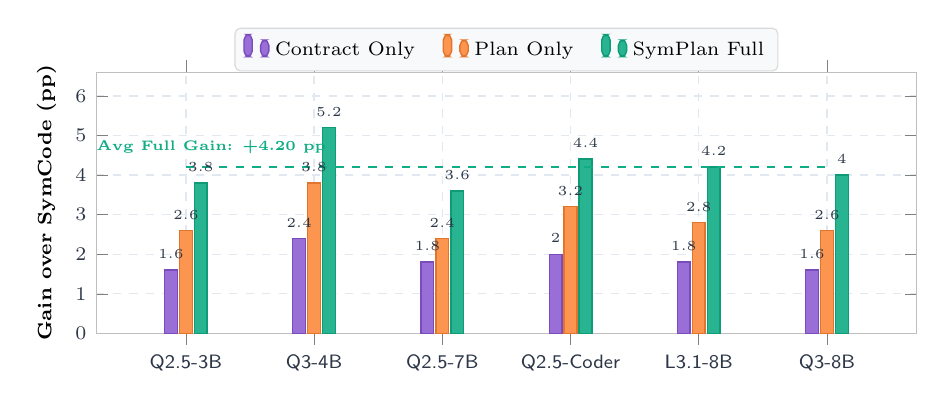
\begin{tikzpicture}
\begin{axis}[
    ybar=0.8pt,
    bar width=4.6pt,
    width=0.99\columnwidth,
    height=4.9cm,
    ymin=0,
    ymax=6.6,
    ytick={0, 1, 2, 3, 4, 5, 6},
    ylabel={\scriptsize\textbf{Gain over SymCode (pp)}},
    symbolic x coords={Q2.5-3B, Q3-4B, Q2.5-7B, Q2.5-Coder, L3.1-8B, Q3-8B},
    xtick=data,
    enlarge x limits=0.14,
    grid=major,
    grid style={draw=chart_grid, line width=0.5pt, dashed},
    axis line style={draw=gray!50},
    x tick label style={font=\scriptsize\sffamily, text=chart_text},
    y tick label style={font=\scriptsize\sffamily, text=chart_text},
    nodes near coords,
    nodes near coords style={font=\fontsize{4.5pt}{5.0pt}\selectfont\bfseries, text=chart_text, yshift=0.5pt},
    legend style={
        at={(0.5,1.17)},
        anchor=north,
        legend columns=3,
        font=\scriptsize,
        draw=gray!30,
        fill=boxgray,
        rounded corners=2pt,
        /tikz/every even column/.append style={column sep=8pt}
    }
]
\addplot[fill=color_contract!85, draw=color_contract!90!black, line width=0.5pt] coordinates {
    (Q2.5-3B, 1.60) (Q3-4B, 2.40) (Q2.5-7B, 1.80) (Q2.5-Coder, 2.00) (L3.1-8B, 1.80) (Q3-8B, 1.60)
};
\addplot[fill=color_plan!85, draw=color_plan!90!black, line width=0.5pt] coordinates {
    (Q2.5-3B, 2.60) (Q3-4B, 3.80) (Q2.5-7B, 2.40) (Q2.5-Coder, 3.20) (L3.1-8B, 2.80) (Q3-8B, 2.60)
};
\addplot[fill=color_symplan!90, draw=color_symplan!90!black, line width=0.5pt] coordinates {
    (Q2.5-3B, 3.80) (Q3-4B, 5.20) (Q2.5-7B, 3.60) (Q2.5-Coder, 4.40) (L3.1-8B, 4.20) (Q3-8B, 4.00)
};
\draw[dashed, color_symplan, line width=0.7pt] (axis cs:Q2.5-3B,4.20) -- (axis cs:Q3-8B,4.20) node[pos=0.04, above=1pt, font=\fontsize{5pt}{6pt}\selectfont\bfseries, text=color_symplan] {Avg Full Gain: +4.20 pp};
\legend{Contract Only, Plan Only, SymPlan Full}
\end{axis}
\end{tikzpicture}
\caption{Accuracy gains over SymCode~\cite{nezhad2025symcode} (percentage points) in the component ablation across all six models on MATH-500. Dashed line denotes the mean full-framework gain ($+4.20$ pp).}
\label{fig:ablation}
\end{figure}

As shown in Fig.~\ref{fig:ablation}, both components independently enhance mathematical reasoning over monolithic SymCode, with algorithmic planning providing the stronger individual benefit ($+2.40\%$ to $+3.80\%$). Crucially, combining fused target contracts with algorithmic planning and anti-regression ranking consistently yields the highest accuracy across every single model ($+3.60\%$ to $+5.20\%$). The target contract prevents type and cardinality mismatch, while the plan structures symbolic transformation.

\subsection{Quantitative Error Analysis and Diagnostics}
\label{sec:error_analysis}

To move beyond anecdotal observations, we conduct a systematic quantitative categorization of all failure instances across the 3,000 problem evaluations (6 models $\times$ 500 problems on MATH-500), summarized in Table~\ref{tab:error_breakdown}.

\begin{table}[t]
\centering
\caption{Quantitative failure mode comparison between SymCode and SymPlan across all 3,000 problem evaluations on MATH-500.}
\label{tab:error_breakdown}
\resizebox{\columnwidth}{!}{%
\begin{tabular}{lcccc}
\toprule
\rowcolor{headergray}
\textbf{Failure Category} & \textbf{SymCode} & \textbf{SymPlan} & \textbf{Net Reduction} & \textbf{Rel. Reduction} \\
\midrule
Execution Failures (Syntax/Crash) & 485 (16.2\%) & 303 (10.1\%) & -182 & \textbf{-37.5\%} \\
Format / Type Mismatches & 515 (17.2\%) & 394 (13.1\%) & -121 & \textbf{-23.5\%} \\
Semantic Misformulations & 974 (32.5\%) & 969 (32.3\%) & -5 & -0.5\% \\
\midrule
\rowcolor{ourgreen}
\textbf{Total Incorrect Solutions} & 1489 (49.6\%) & 1363 (45.4\%) & -126 & \textbf{-8.5\%} \\
\bottomrule
\end{tabular}}
\end{table}

As shown in Table~\ref{tab:error_breakdown}, SymPlan achieves a net reduction of $126$ total errors (an $8.5\%$ relative reduction in overall failure rate). Crucially, the diagnostic breakdown reveals the exact mechanisms responsible for this improvement:

\textbf{1. Reduction in Execution Failures (-37.5\%).} Monolithic SymCode suffered 485 execution crashes ($16.2\%$ of all runs), where models generated invalid syntax, imported non-existent library symbols, or triggered unhandled runtime exceptions. SymPlan reduces these failures to 303 ($10.1\%$), a $37.5\%$ relative drop. By constraining generation with pre-defined SymPy templates and exact fraction rules (\texttt{sp.Rational(p, q)} integer limits), SymPlan shields compact models from library API pitfalls.

\textbf{2. Mitigation of Format and Type Mismatches (-23.5\%).} Format mismatches (where models output unboxed text, template artifacts, or raw solution sets when an integer count is requested) dropped from 515 instances in SymCode to 394 in SymPlan, representing a $23.5\%$ reduction. Explicitly establishing the type contract $\Omega \in \{\texttt{number}, \texttt{text}, \texttt{tuple}, \texttt{set}, \texttt{symbolic}\}$ during the fused planning turn directly guides models to output integer cardinality rather than element enumerations.

\textbf{3. Invariance in Semantic Misformulation: Boundaries of Structural Scaffolding.} Importantly, semantic misformulation remains nearly unchanged between the two approaches ($974 \to 969$ instances, or $32.5\% \to 32.3\%$, representing a negligible $-0.5\%$ difference). Rather than an operational flaw, this invariance represents a central scientific finding: the proposed neurosymbolic scaffolding primarily resolves execution, interface alignment, and structural representation failures rather than fundamentally altering mathematical concept acquisition in compact models. When a compact language model fundamentally lacks the conceptual mathematical intuition required to solve a problem (as is frequently the case on advanced Level-5 competition questions), explicit planning organizes the solver's formal structure but cannot synthesize missing domain theory. In these extreme non-constructive settings, programmatic execution reaches its theoretical ceiling, indicating that extending reasoning to formal interactive proof assistants (such as Lean) represents the necessary next frontier.

\section{Conclusion}

In this paper, we presented SymPlan, an inspectable neurosymbolic framework tailored for mathematical reasoning in compact open-weight language models. By decomposing monolithic symbolic generation into a fused target-planning contract, contract-guided SymPy code synthesis, and targeted debugging with anti-regression selection, SymPlan directly mitigates semantic misformulation, domain omission, and repair regressions. Comprehensive evaluations across six diverse models (spanning 3B to 8B parameters) on the full MATH-500 benchmark demonstrate uniform accuracy improvements of $+3.60\%$ to $+5.20\%$ over SymCode and up to $+23.20\%$ over Chain-of-Thought, alongside a $+6.07\%$ increase in execution success rate, all without parameter fine-tuning.

In future work, we plan to extend SymPlan to multimodal mathematical reasoning involving geometric diagrams, as well as investigate the integration of interactive formal theorem provers (such as Lean) to verify open-ended deductive proofs on edge devices.

\bibliographystyle{splncs04}
\bibliography{cite}

\end{document}
